\documentclass[10pt]{article}
\usepackage[a4paper,margin=18mm]{geometry}
\usepackage{amsmath,amssymb,graphicx,booktabs,hyperref}
\hypersetup{hidelinks}
\title{Elastic contact forces and independent angular impulses\\Completed sphere--plane verification}
\author{Rigid Body Collisions research prototype}\date{5 October 2026}
\begin{document}\emergencystretch=2em\maketitle
All ten original cases now satisfy their unchanged gates. The complete predeclared study verifies 18 of 18 cases over 54 histories, with no rejected attempts. Earlier failed studies remain archived. These are synthetic constitutive hypotheses and mathematical/numerical verification cases: no measured rubber calibration, new friction law, or arbitrary-body native coupling is claimed. Frozen source: \texttt{7c3a47c46d7c}.
\section*{A generalized impulse includes an independent couple}
For a solid sphere, $\mathbb I=2mR^2/5$. With a fixed-plane normal $\hat n$ directed into the admissible half-space, use the reference lever $r=-R\hat n$. The cross-product matrix and contact velocity are
\[
r\wedge=\begin{bmatrix}0&-r_z&r_y\\r_z&0&-r_x\\-r_y&r_x&0\end{bmatrix},\qquad
v_c=v+(r\wedge)^\mathsf T\omega.
\]
The independent angular impulse $\Delta L$ is separate from the angular momentum generated by a point force:
\[
m\Delta v=\Delta p+mg\,\Delta t,\qquad
\mathbb I\Delta\omega=(r\wedge)\Delta p+\Delta L.
\]
For an instantaneous fixed-lever impulse without gravity, define
\[
V=\begin{bmatrix}v_c\\\omega\end{bmatrix},\quad
\Delta P=\begin{bmatrix}\Delta p\\\Delta L\end{bmatrix},\quad
\Delta V=M\Delta P,\quad
M=\begin{bmatrix}1/m-(r\wedge)\mathbb I^{-1}(r\wedge)&-(r\wedge)\mathbb I^{-1}\\
\mathbb I^{-1}(r\wedge)&\mathbb I^{-1}\end{bmatrix}.
\]
Scalar matrix additions implicitly multiply the identity. The mixed-unit vector is bookkeeping; $V^\mathsf T\Delta P$ still has energy units. The kinetic change is
\[
\Delta E_k=(V^-)^\mathsf T\Delta P+\tfrac12\Delta P^\mathsf T M\Delta P.
\]
A normal-axis spin change requires $\Delta L$: $(r\wedge)\Delta p$ has zero component along $\hat n$.
\section*{One potential, a shared yield budget, and a complete energy ledger}
Let $h=(q_1,q_2,a\theta)^\mathsf T$, $K=\operatorname{diag}(k_t,k_t,k_\theta/a^2)$, $f=(\delta/R)^p$, and $\delta=\max(0,R-\hat n\cdot x+d)$. Here $a$ is an effective contact length, with no required meshed patch. The two supported exponents are $p=2$ for the weighted material and $p=0$ for the linear benchmark:
\[
U=\tfrac12k_n\delta^2+U_h,\quad U_h=\tfrac12f h^\mathsf TKh,\quad
F_n=k_n\delta+c_n\max(0,\dot\delta)+pU_h/\delta.
\]
\[
F_t=-fk_tq,\quad\tau_n=-fk_\theta\theta,\quad
\sqrt{\|F_t\|^2+(\tau_n/a)^2}\leq\mu k_n\delta\leq\mu F_n.
\]
The shared ellipsoid is a phenomenological capacity approximation, not an exact traction surface for every pressure distribution. One coefficient covers stick and slide. Let $e=fKh$, $s=e/\|e\|$, $u=(T^\mathsf Tv_c,a\hat n\cdot\omega)^\mathsf T$. Associated plastic flow removes outward yield loading:
\[
\dot h=u-\lambda s,\quad
\lambda=\max\left(0,\frac{s\cdot[p(\dot\delta/\delta)e+fKu]-\mu k_n\dot\delta}{f\,s^\mathsf TKs}\right),\quad
\dot D=c_n\max(0,\dot\delta)\dot\delta+\lambda\|e\|\geq0.
\]
Consequently, including gravity,
\[
\frac{d}{dt}\left(\tfrac12m\|v\|^2+\tfrac12\mathbb I\|\omega\|^2-mg\cdot x+U+D\right)=0.
\]
\newpage
\section*{Numerical repair and material-preserving effort selection}
The earlier rejected high-spin, low-friction case exhausted 20,000 RHS evaluations when explicit integration repeatedly switched yield branches at individual stages. The revised solver follows elastic or yielded modes between exact yield, release and lift-off events. Material parameters, the force law and the budget are unchanged. Exact ballistic free motion skips contact evaluations between impacts. A grazing contact with no inward crossing creates no spurious zero-time transitions.

The high-spin weighted case now needs 4,233 evaluations at the finest level: $\Omega_z:10\to5.20433335$ rad/s, $v_z:-1\to1.00371591$ m/s, $D=0.14210701$ J, complete energy residual $1.59\times10^{-14}$ J. Low friction correctly does not reverse this spin. Its negative-spin counterpart has the reflected result.

For $p=0$, zero damping, no prior history, zero gravity during contact and sufficiently large shared capacity, a conditional exact branch uses matched frequencies:
\[
\omega_c=\sqrt{k_n/m},\quad m_t=(1/m+R^2/\mathbb I)^{-1},\quad k_t=m_t\omega_c^2,\quad k_\theta=\mathbb I\omega_c^2.
\]
With incoming normal speed $V_n>0$, tangent contact velocity $u_t$ and normal spin $\Omega_n$, sticking is proved throughout the half-period when
\[
\sqrt{(m_t\|u_t\|)^2+(\mathbb I\Omega_n/a)^2}\leq\mu mV_n.
\]
The exact impulse and duration are
\[
\Delta p=2mV_n\hat n-2m_tu_t,\quad\Delta L=-2\mathbb I\Omega_n\hat n,\quad t_c=\pi/\omega_c.
\]
Otherwise the dispatcher resolves the \emph{same configured material} with history. It never replaces elastic return by an inelastic Coulomb law for speed. Sphere/plane scope, deformation budget and total energy gates apply to both branches.
\par\noindent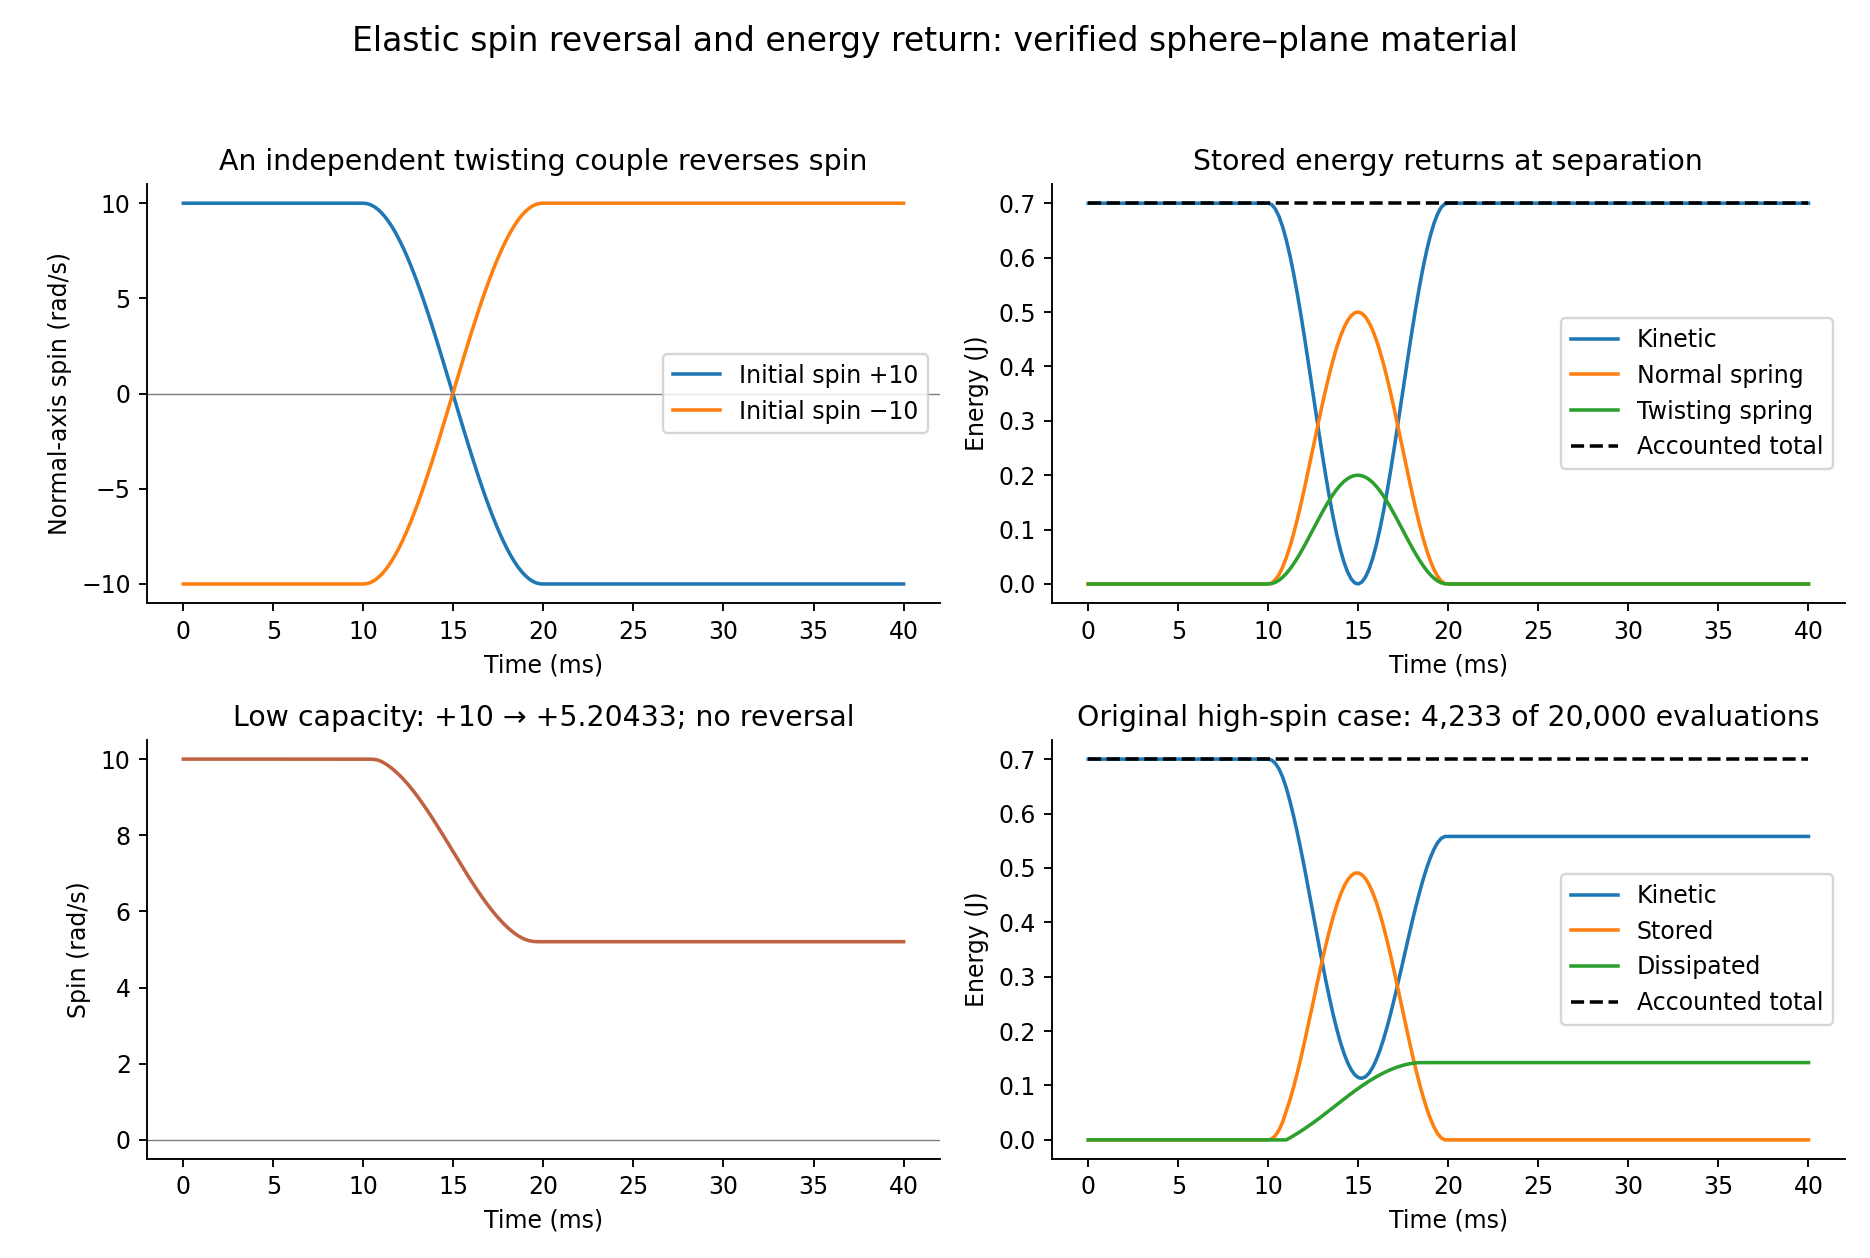
\includegraphics[width=\textwidth]{spin-energy.png}
\newpage
\section*{Continuous bounce sequences and independent evidence}
For the matched elastic contact, a vertical floor--ceiling path undergoes five lift-offs in 0.18 s. Both twist signs reverse at every impact, without resetting the body state. A separate oblique same-floor trajectory under gravity has three bounces: horizontal COM motion, tangent-axis spin and normal-axis spin all alternate. It retains the original $k_n=10^8$ N/m material. Gravity perturbs the ideal contact period, producing a brief resolved yield tail before lift-off. Over three bounces its plastic loss is $2.095\times10^{-6}$ J; its separation-store removal is only $4.89\times10^{-18}$ J. The complete energy residual remains $1.17\times10^{-12}$ J.

An arbitrary oblique floor--ceiling path need not retrace: reversing the plane normal changes tangential force--spin coupling. The verified chained ceiling trajectory is vertical with normal-axis twist; the verified oblique back-and-forth trajectory repeatedly meets the same floor. Additional rolling-couple mechanics would require separate justification and validation.
\par\noindent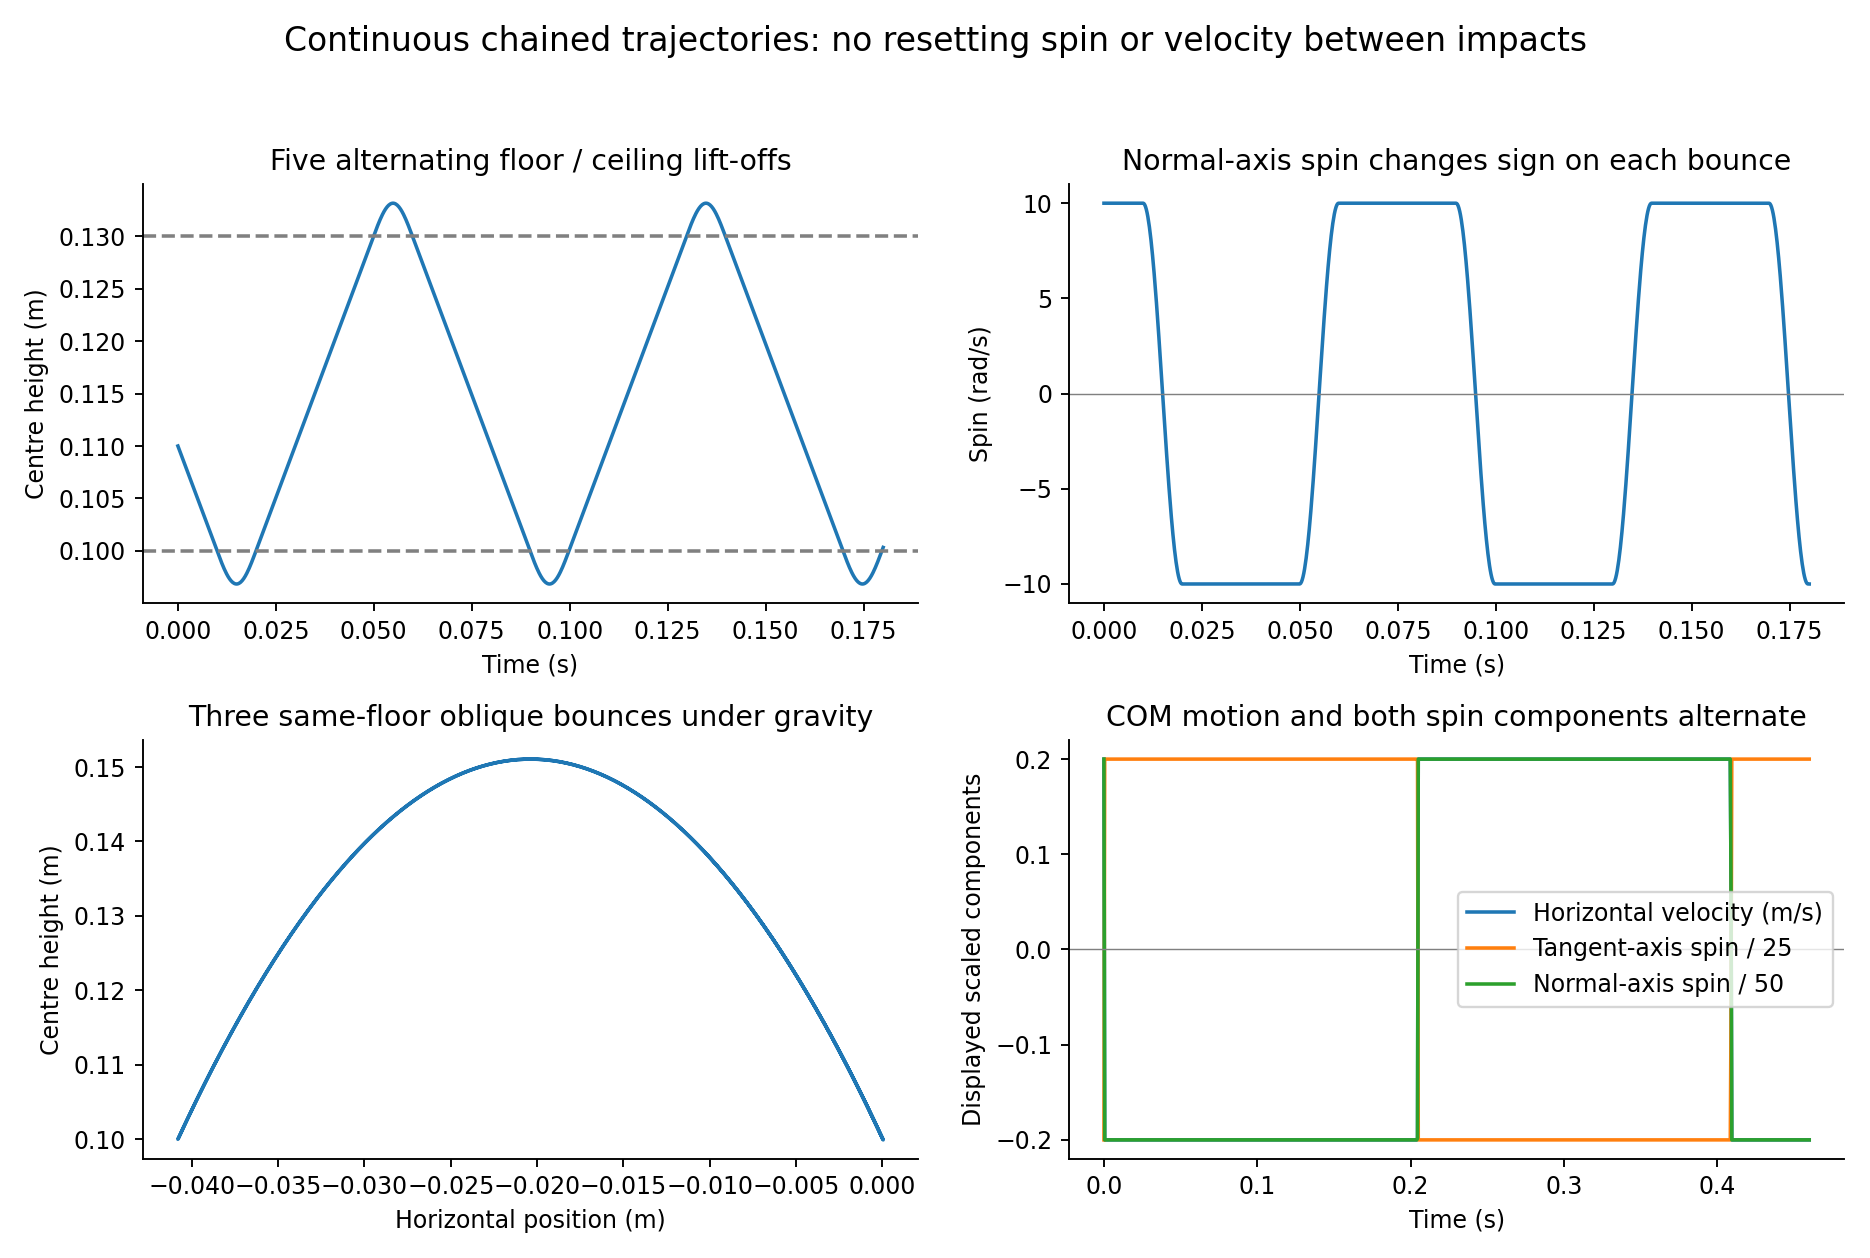
\includegraphics[width=.9\textwidth]{bounces.png}
\begin{center}\footnotesize\begin{tabular}{p{62mm}rrr}\toprule
Case & $\Omega_y,\Omega_z$ (rad/s) & Energy error (J) & RHS\\\midrule
elastic normal axis spin & 0, -10 & 2.9e-14 & 3995 \\
elastic tangent axis spin & -4.2857, 0 & 1.4e-14 & 4214 \\
low friction no spin reversal & 0, 9 & 1.2e-14 & 4210 \\
compression weighted reversal & 0, -1.32682 & 1.5e-14 & 3917 \\
weighted high spin low friction budget & 0, 5.20433 & 1.6e-14 & 4233 \\
same floor oblique mixed positive & 5, -9.99997 & 1.2e-12 & 35196 \\
\bottomrule\end{tabular}\end{center}
The independent audit recomputes sample and accepted-step energy, linear momentum, offset-force versus independent-couple angular momentum, shared capacity, both adjacent refinement edges and every bounce criterion. Dispatchers are replayed from archived source in a clean process. Same-material slow/rapid examples cover 0.01 and 100 m/s in both twist directions. These are checks of an ideal material, not evidence that actual rubber is rate independent or accurate at those speeds. Force peaks are numerical accepted-step/sample diagnostics, not certified continuous suprema. The native arbitrary-shape engine does not yet integrate these independent elastic couples.
\section*{Related mechanics and calibration limits}
\begingroup\small\sloppy
Rod Cross, ``Grip-slip behavior of a bouncing ball'', \emph{American Journal of Physics} 73 (2005), DOI: \href{https://doi.org/10.1119/1.2008299}{10.1119/1.2008299}, demonstrates that friction magnitude alone does not determine elastic spin return. Xydas and Kao, \emph{IJRR} 18 (1999), DOI: \href{https://doi.org/10.1177/02783649922066673}{10.1177/02783649922066673}, discuss soft-contact force/moment capacity. The accompanying retained mechanics review provides qualifications and measured counterexamples. No novelty or publication claim follows solely from the verified examples.
\endgroup
\end{document}
